\documentclass[a4paper,12pt,headsepline]{report}

%----------------- PDF CONFIG ----------------- %
\pdfinfo{    
     /Title (Bachelorthesis) 
     /Subject   (Reactive Programming)    
     /Author  (Felix Scheidel) 
     /Keywords   (Java 8, Reactive Programming, Functional Reactive Programming, RxJava, RxJavaFx)      
} 

\title{Reactive Programming}
\author{Felix Scheidel}
\date{\today}



%----------------- PAKETE INKLUDIEREN ----------------- %

\usepackage{geometry} % Packet für Seitenrandabständex und Einstellung für Seitenränder
\usepackage[ngerman]{babel} % deutsche Silbentrennung

\usepackage{booktabs} %entzerrt die Tabellenzeilen und bietet verschieden dicke Unterteilungslinien
\usepackage{longtable} % Tabellen können sich nicht über mehrere Seiten 
\usepackage{graphicx} % kann LaTeX Grafiken einbinden

\usepackage[utf8]{inputenc} % Umlaute unter Mac werden automatisch gesetzt
\usepackage[T1]{fontenc} % Zeichenencoding
\usepackage{lmodern} % typographische Qualität 
\frenchspacing % Schaltet den zusätzlichen Zwischenraum ab
\usepackage{fix-cm}
\usepackage{hyperref} % verwandelt alle Kapitelüberschriften, Verweise aufs Literaturverzeichnis und andere Querverweise in PDF-Hyperlinks
\usepackage{color}
\usepackage{url}


\usepackage[nottoc]{tocbibind}



% für Listings
\usepackage{listings}
\lstset{numbers=left, numberstyle=\tiny, numbersep=5pt, stepnumber=4, keywordstyle=\color{black}\bfseries\itshape, stringstyle=\ttfamily,showstringspaces=false,basicstyle=\footnotesize,captionpos=b}
\lstset{language=java}



%----------------- FARBEN DEFINIEREN ----------------- %
\definecolor{gray}{gray}{0.95} % Listingsbackground

%----------------- LAYOUT SETZEN ----------------- %
\geometry{left=2cm, right=2cm, top=2.5cm, bottom=2cm}
\linespread {1.25}\selectfont %1.25 da er von Haus aus 1.2 ist und 1,25 * 1,2 = 1,5 isch




%-------##-------##-------##------- ANFANG INHALT -------##-------##-------##-------%
\begin{document}



\pagenumbering{roman} % Seitennummer

%----------------- DECKBLATT -----------------%
 %----------------- KONFIGURATION ----------------- %
\pagestyle{empty} % enthalten keinerlei Kopf oder Fuß 

%----------------- Logo ----------------- %
\begin{figure}[t]
	\centering
	
\includegraphics[width=0.35\textwidth]{Abb/hs-logo} \hspace{2cm}
	
\includegraphics[width=0.35\textwidth]{Abb/pentasys_logo}
\end{figure}

%----------------- INHALT ----------------- %

\begin{center}
\Large Hochschule Kaiserslautern \\
\normalsize \textsc{- Fachbereich Informatik und Microsystemtechnik -} \\

% Whitespace
\vspace{105 pt}

\Huge Der Titel der Arbeit \\ 
\normalsize
\vspace{20 pt}

Abschlussarbeit zur Erlangung des akademischen Grades \\ 
Bachelor of Science (B.Sc.) 

\vspace{75 pt}


vorgelegt von \\
\vspace{5 pt}
Vorname Nachname \\
12345
\vspace{115 pt}

\begin{tabular}[h]{p{4cm}l l}
	Betreuer Hochschule: & Prof. Dr. \\
	Betreuer PENTASYS: & B. Sc. 
\end{tabular}


\end{center}

 
%----------------- ABSTRACT -----------------%
 %----------------- KONFIGURATION ----------------- %
\pagestyle{empty} % enthalten keinerlei Kopf oder Fuß

\section*{Zusammenfassung} % (fold)
\label{cha:zusammenfassung}
In dieser wissenschaftlichen Arbeit wird das Programmierparadigma \textit{Reactive Programming} behandelt. Reactive Programming verbindet die Eigenschafen für asychonres, nicht blockierendes Verarbeiten von Datenströmen. Zu Beginn wird geklärt wie dieses Paradigma in den Kontext der Softwareentwicklung eingeordnet werden kann und wie es sich von Reactive Systems unterscheidet. Anschließend beschäftigt sich diese Arbeit mit den Bestandteilen wie dem Observer Pattern und dem Back Pressure, die dieses asynchrone und nicht blockierende Verhalten generieren. Zusammen bilden sie die Reactive Streams welche ebenfalls genauer erläutern werden. Auch wird eine bereits vorhandene Implementierung in Form der RxJava2 Bibliothek im Detail betrachtet. Es werden Eigenschaften wie Synchronität oder Nebenläufigkeit beschrieben. Weiterhin wird auf die grundlegenden Klassen wie Observables oder Schedulers genauer eingegangen und deren Beschreibungen werden durch Codebeispiele unterstützt. Es folgt eine Implementierung eines Systemmonitors als Beispielapplikation welche die RxJava2 Bibliothek verwendet und einige vorab besprochene Methoden genauer bahandelt. Abschließend wird evaluiert wo Reactive Programming seine Vorteile hat und in welchen Anwendungsbereichen sich dieses Paradigma etablieren kann. Diese Einschätzung legt nah, dass die wahrscheinlich sinnvollsten Gebiete die Arbeit mit REST-Schnittstellen, Microservice-Architekturen und sehr I/O basierte Anwendungen sein werden.


\vspace*{1,5cm}
\section*{Abstract} % (fold)
\label{cha:abtract}
This scientfic work is treating the programming paradigm \textit{Reactive Programming}. This paradigm combines the attributes for asynchronous and non-blocking processing of datastreams. At first Reacitve Programming is classified into the context of software development and the difference to Reactive Systems is exposed. Afterwards this work explains different parts like Observer Pattern or Back Pressure which are necessary to create the asynchronous and non-blocking behavior. Theses parts put together the Reactive Streams, which also get explained in this work. Furthermore an implementation of the already existing library RxJava2 gets discussed in detail. Characteristics like synchronicity and concurrency get described. There will be a closer look into the base classes like Observables and Schedulers accompanied with some coding examples. Ensuing there is an implementation of a system monitoring tool using the RxJava2 library and showing of some of the preceding methods. Finally an evaluation of the benefits of the Reactive Programming paradigm takes place, explaining which area of application this paradigm has its best use. The resulting estimation sees REST-Interfaces, the Microservice Architecture and very I/O heavy applications as the most meaningful areas of effect for Reactive Programming.
 


 
 
%----------------- VERZEICHNISSE -----------------%
\tableofcontents % Inhaltverzeichnis

\pagestyle{plain} % zurueck setzen von roemische seitenanzahl


%----------------- KAPITEL : EINFÜHRUNG  ----------------- %
\pagenumbering{arabic}
\chapter{Einf"uhrung}
\label{cha:einfuehrung}

Lorem ipsum dolor sit amet, consetetur sadipscing elitr, sed diam nonumy eirmod tempor invidunt ut labore et dolore magna aliquyam erat, sed diam voluptua. At vero eos et accusam et justo duo dolores et ea rebum. Stet clita kasd gubergren, no sea takimata sanctus est Lorem ipsum dolor sit amet. Lorem ipsum dolor sit amet, consetetur sadipscing elitr, sed diam nonumy eirmod tempor invidunt ut labore et dolore magna aliquyam erat, sed diam voluptua. At vero eos et accusam et justo duo dolores et ea rebum. Stet clita kasd gubergren, no sea takimata sanctus est Lorem ipsum dolor sit amet.


%----------------- KAPITEL : WAS IST RP  ----------------- %	
\chapter{Was ist Reactive Programming}\label{was_ist_reactive_programming}
Ist man neu in der Domäne von reaktiver Entwicklung stellt man schnell fest, dass allerhand mögliche Definitionen und Beschreibungen findet was Reactive Programming denn zu sein scheint. Bevor jedoch hier eine Definition erläutert wird, muss zwischen unterschiedlichen Begrifflichkeiten differenziert werden: \textit{Reactive Systems, Functional Reactive Programming} und natürlich \textit{Reactive Programming}. Vorab wird jedoch ergründet worum es sich grundlegend handelt und wieso es zur heutigen Zeit von Relevanz ist über die möglichen Verwendung von \textit{reactive} zu sprechen.
\section{Was bedeutet \textit{"reactive"} im Kontext der Softwareentwicklung}
Wie die Wortherkunft verlauten lässt, wird etwas als reaktiv bezeichnet, wenn eine Reaktion durch eine vorangegangene Aktion ausgelöst wird. Bei diesen Aktionen handelt es sich meist um Veränderungen an verwendeten Daten und stattfindende Ereignisse(\textit{Events}). Eine gutes Beispiel zur Veranschaulichung ist die Benutzeroberfläche(\textit{GUI}). Ein Benutzer bestätigt eine vorgenommene Eingabe durch das klicken eines Button innerhalb der GUI. Dieses Event sorgt dafür, dass die Applikation einen vorgegebenen Vorgang ausführt. Dieses Vorgehen sorgt in der klassischen objektorientierten Programmierweise mit sequentiellem Ablauf sowie dem imperativen Ansatz grundsätzlich für ein stetig wachsendes Maß an Komplexität. Durch die unterschiedlichen Events die innerhalb der GUI ausgelöst werden können(Mausklick, Tastendruck, usw.) ist ein klassischer imperativer sowie sequentieller Ablauf den Programmcodes nicht realistisch, da kein Entwickler weiß, in welcher Reihenfolge und zu welchem Zeitpunkt ein beziehungsweise welches Event ausgelöst wird. Somit spielt hier die \textit{Inversion of Control}\footnote{Vgl. \cite{MartinFowler.2005}, https://martinfowler.com/bliki/InversionOfControl.html.}, also das Umkehren der Kontrolle, eine große Rolle. Diese besagt, dass nicht der geschrieben Code den Ablauf beschreibt, sondern die Kontrolle bei dem Framework\footnote{In diesem Fall ein Framework für das Realisieren einer GUI. Vgl. \cite{wiki.guilist}.}, welches für die Interaktion zuständig ist, liegt, und dieses entscheidet wiederum wie und wann auf ein Event reagiert wird. Im Code spiegelt sich das dadurch wider, das mögliche Reaktionen, meist als Methoden oder Funktionen realisiert, an die mögliche eintreffenden Ereignisse gebunden werden. Dies geschieht über so genannte Event-Handler beziehungsweise Event-Listener oder über die Verwendung von Callbacks\footnote{TODO Beispiel Event-Handler -> ActionEvent, Click on Button; Quellen angeben und Beschreibung zu Beiden Codebeispielen}. Ein bewährtes und klassisches Vorgehen bei Anwendungsanforderungen dieser Art ist das schon 1994 von Erich Gamma und seinen Mitstreitern beschriebenes Entwurfsmuster\footnote{\cite{Gamma.2011}: Dieses Buch beschreibt viele noch heute verwendete Entwurfsmuster. Die Autoren sind in die Geschichte als die Gang Of Four (\textit{GoF}) eingegangen.}, dem \textit{Observer-Pattern}\footnote{Hier Beispiel vom OP sowie Übersetzung Beobachtermuster; Observer Pattern und Erklärung}. Man betrachtet hier grundlegend zwei Ansätze: \textit{push}  und \textit{pull}. \footnote{Hier gute Beispiele für push und pull Variante}. Auch hier lässt sich wieder die GUI als guten Beispiel heran ziehen. Man betrachtet eine Oberfläche welche die Temperatur im Raum anzeigt. Die Temperatur wird als Zahl in Grad Celsius sowie graphisch in einem Balken dargestellt. Obwohl beide Elemente auf die selben Daten zugreifen, stehen programmatisch die Objekte in keine Zusammenhang. Um nun das Beobachtermuster zu implementieren, muss der sich ändernde Wert der zum Beispiel von einem Temperatursensor gemessen wird regelmäßig aktualisiert beobachtet werden. Das Objekt, welches den Temperaturwert inne hält wird somit als beobachtbar deklariert, die beiden Objekte, die Ausgabe per Zahlenwert und der graphische Balken, werden bei diesem Objekt als Beobachter registriert. Wenn man den push-Ansatz verfolgt, wird jedem Beobachter benachrichtigt und das Objekt mit den geänderten Daten steht dem Beobachter zur Verfügung. Verfolgt man den pull-Ansatz, werden die Beobachter nur kurz darüber informiert, dass sich Werte innerhalb des zu beobachtenden Objekts geändert haben, müssen jedoch aktiv anfragen um die geänderten Werte zu erhalten. Je nach Vorgehen ergeben sich Vor- und Nachteile. Der push-Ansatz steht eher für lose Kopplung, da der Beobachter keine Details zu dem zu beobachteten Objekt braucht. Jedoch sinkt dadurch die Flexibilität, da Beobachterschnittstellen exakter beschrieben werden müssen damit der Beobachtete weiß welche Information weiter gereicht werden sollen. Die Kopplung im Vergleich zum pull-Ansatz ist nicht wirklich lose, da jeder Beobachter wissen muss, welche Daten das observierte Objekt repräsentiert und wie auf diese Daten zugegriffen werden kann. Jedoch findet sich hier die Flexibilität wieder, da jeder Beobachter wenn er Information braucht, exakt diese Daten abrufen kann und sich nicht auf die korrekte Datenverteilung des Beobachteten verlassen muss. \\ Nach diesem Abschnitt sollte soweit klar sein, wie man ein reaktives Verhalten mit den schon bekannten Bordmitteln realisiert.
\subsection{Differenzierung zwischen Reactive Proramming und Reactive Systems}
Das zuvor angesprochene Verhalten bezieht sich nur auf ein Beispiel. Wie jedoch wirkt es sich aus, wenn eine komplette Anwendung unter Verwendung dieses Stils entwickelt wird? Wie verhält es sich weiter wenn mehrere Teile reaktiv funktionieren und kommunizieren sollen? Der grundlegende Gedanke reaktiver Systeme wurde schon im Jahre 1985 in einem Paper von D. Harel und A. Pnueli beschrieben\footnote{\cite{Harel1985}}. Zur heutigen Zeit jedoch bezieht man sich bei Richtlinien zur Gestaltung reaktiver Anwendungen eher auf das Reactive Manifesto\footnote{\cite{Boner.} -> ebenso Bild von Manifest einfügen. Deutsches Manifest in Quellen verlinken}. Laut Jonas Bonér und den vielen Unterstützern sind vier Bestandteile essentiell, damit eine Anwendung die Anforderung erfüllt um sich reaktiv zu verhalten. Die Ansicht des Manifest stützt sich auf einen Architektur- beziehungsweise Designstil und soll als Grundlage zur Entwicklung Reaktiver Systeme dienen. Die folgenden Erklärungen sind dem Manifest entnommen und sollen einen Verständnis zu den vier Eigenschaften bieten. Wie in diesem beschrieben sind Reaktive Systeme:
\begin{itemize}
	\item \textbf{Antwortbereit (engl. responsive):}\\ Ein System muss immer zeitgerecht antworten. Die Antwortbereitschaft ist die Grundlage für die Benutzbarkeit besagten Systems. Ebenso wird um eine Fehlerbehandlung durchführen zu können eine geregelte Antwortbereitschaft vorausgesetzt.
	\item \textbf{Widerstandsfähig (engl. resilient):}\\ Ein System muss auch bei Ausfällen die Antwortbereitschaft aufrecht erhalten. Die wird durch Replikation der Funktionalität, der Isolation von Komponenten sowie dem Delegieren von Verantwortung erzielt. 
	\item \textbf{Elastisch (engl. elastic):}\\ Das System muss bei sich ändernden Lasten die Funktionalität und Antwortbereitschaft aufrecht erhalten. Ressourcen müssen den auftretenden Lasten, ob steigend oder sinken, angepasst werden können.Ebenso müssen Engpässe innerhalb des Systems unterbunden werden um die Elastizität zu bewahren.
	\item \textbf{Nachrichtenorientiert (engl. message driven):}\\ Ein loses System soll zur Kommunikation zwischen den Komponenten auf asynchrone, ortsunabhängige Nachrichtenübermittlung zurück greifen. Somit ist nicht relevant auf welchen Rechner die einzelnen Komponenten ausgeführt werden, wodurch wiederum eine gute Skalierbarkeit entsteht.
\end{itemize}
Das Manifest erwähnt jedoch in keinster Weise den Zusammenhang von Systemen zum reaktiven Programmieren. Auch aus diesem Grund hat Jonas Bonér einen weiteren Artikel\footnote{\cite{Boner.2014}} verfasst, der sich dieser Thematik annimmt. Die grundlegenden Unterschiede wurde in dem Artikel wie folgt zusammengefasst.
\begin{itemize}
	\item Reactive Programming ist eine Teilmenge von Reaktiven Systemen auf Implementierungsebene
	\item Reactive Programming liefert Leistung und effektive Ressourcennutzung auf Komponentenebene, speziell für Softwareentwickler
	\item Reaktive Systeme hingegen bieten Robustheit und Elastizität auf Systemebene zur Gestaltung von Cloud-kompatiblen oder verteilten Anwendungen, speziell für Softwarearchitekten oder DevOps
	\item Es ist von großem Vorteil reaktives Programmieren innerhalb der Bestandteile von reaktiven Systemen zu verwenden
	\item Es is ebenso von Vorteil reaktive Systeme zur Interaktion zwischen reaktiv programmierten Komponenten zu verwenden
\end{itemize}
Wie aus diesen Punkten klar wird, liegt also der genau Unterschied zwischen reaktivem Programmieren und reaktiven System aus welcher Perspektive die Betrachtung stattfindet. Architektonisch wird von Systemen gesprochen, die innerhalb und zur Interaktion mit anderen reaktiv reagiert. Betrachtet man das Ganze aus Entwicklersicht eine Komponente, kann diese unter Zuhilfenahme von reaktivem Programmieren für ein asynchrones, paralleles Verhalten entwickelt werden. Wie Jonas Bonér schon schreibt, ist das Zusammenspiel beider sehr oft hilfreich um das gewünschte Ziel zu erreichen. Ein weiterer wichtiger Punkt ist die Unterscheidung von \textit{ereignisorientiert} zu \textit{nachrichtenorientiert}. Nachrichten werden auf Systemebene genutzt. im Gegensatz zu Ereignissen sind Nachrichten klar an einen Empfänger adressiert. Ereignisse treten auf und müssen beobachtet werden um das gewünschte Resultat zu erzielen. Nachrichten sind somit gut geeignet bekannte Empfänger in einem verteilten System, zum Beispiel über das Netzwerk, zu kontaktieren. Innerhalb der Komponente besteht die Funktion (man denke hier wieder an die Nutzeroberfläche) oft aus der Reaktion auf Ereignisse unterschiedlicher Art die direkt in der Komponente verarbeitet werden sollen. Somit herrscht hier ein Ereignis-getriebenes Verhalten. 

\section{Reactive Programming vs. Functional Reactive Programming}
Auf der Suche nach einer Definition zu Reactive Programming stößt man oft auf es Begriff Functional Reactive Programming. Teilweise werden die Begriffe sogar synonym verwendet\footnote{Vgl.: \cite{Nurkiewicz.2017}, Seite 2.}. Grundlegend betrachtet man bei den bekannten Programmierparadigmen zwischen imperativen und deklarativen Paradigmen, wobei zum Beispiel die Objektorientierte Programmierung im imperativen und funktionale Programmierung im deklarativen Bereich angesiedelt wird. Funktionale Programmierung zeichnet vor allem die Nutzung des Lambda-Kalküls aus. Dadurch wird programmatisch nicht die Frage nach dem \textit{Wie} gelöst, sondern ein Vorgang wird mit mathematischen Funktionen beschrieben\footnote{Verweis auf Lambda-Kalkül}. Wird eine funktionale Programmiersprache nun um den relevanten Faktor Zeit erweitert kann ein reaktives Verhalten beschrieben werden. Diese Art der Realisierung nennt man \textit{Functional Reactive Programming}\footnote{\cite{frp.haskell}}. Somit kann das FRP als Teilmenge des Paradigma der reaktiven Programmierung angesehen werden. Die Verwechslung der Begriffe entsteht wenn man sich zum Beispiel Java 8 anschaut. Mit Java 8 nahm die Klasse der Funktionen sowie die Lambda-Ausdrücke Einzug in die OO Programmiersprache\footnote{Noch Verweis suchen: Viele weitere bekannte Programmiersprache wie C\# z.B. unterstützen Lambdas ebenso} Java. Dadurch wird ein ähnliches Verhalten der Funktionalen Programmierung reproduziert. Somit kann innerhalb von Java reaktiv unter Zuhilfenahme von funktionalen Methodiken entwickelt werden. Der Unterschied findet sich also genau an der Stelle, dass funktionale Eigenschaften zwar in Java vorhanden sind, dadurch Java allerdings nicht als funktionale Programmiersprache verstanden werden kann, denn auch innerhalb der Objektorientierung kann auf dem imperativen Weg ein reaktives Verhalten entwickelt werden. Reactive Programming kann somit als eine Abstraktion gesehen werden, die sich über die Vorhandenen Paradigmen erstreckt und je nach Situation und Anwendungsbereich auf andere Programmierstile zurück greift. 

\section{Wie wird Reactive Programming realisiert?}
Es wurde berichtet was allgemein unter einem reaktiven Verhalten verstanden wird. Ebenso wurde die Begrifflichkeiten und Zusammenhängen zwischen Reactive Programming, Reactive Systems und Functional Reactive Programming erläutert. Es stellt sich jedoch noch die Frage wieso aktuell die Reaktivität von Applikation stark gefordert wird und wie eine Umsetzung davon aussieht. Durch große Datenraten, Datenmengen und vielen vernetzten Geräte und Dienste die zur heutigen Zeit in Umlauf sind, entstehen viele Informationen die verarbeitet werden können beziehungsweise müssen. Durch die vielen Berechnungen und Verarbeitungsschritte die dafür nötig sind, spielt hier das Gesetz von Amdahl eine große Rolle\footnote{Vgl. \cite{Amdahl.}. Es handelt sich um einen Reprint in der IEEE SSCS News. Auf diesem von Amdahl verfassten Original resultiert das gleichnamige Gesetz.}. Dieses besagt, dass nie alle Teile eines Programms parallel ausgeführt werden können. Somit lohnt es sich, denn Ablauf in einen sequentiellen und einen parallelen Teil zu zerlegen. Die Blockade die somit noch bleibt, sind die Programmteile die sequentiell abgearbeitet werden müssen und nicht weiter optmiert werden können. Reactive Programming versucht nun eine Lösung abzubilden die den Ablauf innerhalb des parallelen Teils vereinfacht und beschleunigt um eine möglichst geringe Latenz und große Flexibilität und Reaktionsfreudigkeit eines Programms widerzuspiegeln. Ein Ansatz diese Lösung zu realisieren ist die Verwendung von Datenströmen. Die Stream-Api wurde wie die Lambda-Funktionalität mit Java 8 eingeführt. Sich veränderte oder neue Daten werden als Ströme betrachtet, die unter Beobachtung stehen und Änderungen sowie Bearbeitung der Daten asynchron und parallel zu den anderen Funktionen einer Anwendung ausgeführt werden können. Damit dieses Verfahren der Datenverarbeitung funktioniert, sind einige Konzepte zu beachten.
\subsection{Datenströme- Streams}
Das Konzept der Streams stellt eine Abstraktion für Folgen von Bearbeitungsschritten auf Daten dar\footnote{Vgl. \cite{Inden.2015}, Seite 42.}. Streams erinnern an Collections sind jedoch nur einmal traversierbar und nehmen keine direkten Speicherung der Daten vor. Collections können auch als Datenströme respräsentiert werden. Nahe liegt die verbreitete Analogie der Fließbandverarbeitung. Man hat eine Menge von Objekten die nacheinander gewissen Operationen unterzogen werden. Diese wird einmalig durchgeführt und die Zwischenergebnisse bleiben nicht vorhanden. 
\subsection{Massenverarbeitung - Bulk Operations}
Diese Operationen gelten als funktional in sind seit Java 8 auf Collections sowie Streams anwendbar. Diese Operation müssen nicht separat implementiert werden und können direkt auf Collections oder Streams ausgeführt werden\footnote{Beispiel Bulk Operation}. Somit kann durch eine Operation zum Beispiel eine Veränderung an jedem Objekt einer Liste ausgeführt werden, oder eben auf jedem Objekt welches einen Datenstrom durchquert. Die Operation können verkettet werden. Zu beachtet ist, dass jede Operation auf einer Kopie des eigentlichen Objekts ausgeführt wird, also bleibt zum Beispiel die Liste unverändert wenn man solch eine Massenoperation auf die Elemente der List ausführt. Als Ergebnis wird eine modifizierte Kopie der ursprünglichen Liste geliefert. Auch bei einer Verkettung wird immer nur eine Kopie des Eingangsobjekts modifiziert und weiter gereicht. Dies gilt äquivalent auch für Streams. Erwähnung sollte noch die unterschiedliche Art von Operation finden. Es wird zwischen drei Arten von Operationen unterschieden: \textit{Erzeugung}, \textit{Berechnung} und \textit{Ergebnisermittlung}\footnote{Vgl.: \cite{Inden.2015}, Seite 42f.} die sich wie folgt abbilden lassen: 
\begin{displaymath}
	\underbrace{Quelle \Rightarrow STREAM}_{Erstellung} \Rightarrow \underbrace{OP_{1} \Rightarrow OP_{2} \Rightarrow ... \Rightarrow OP_{n}}_{Berechnung} \Rightarrow \underbrace{Ergebnis}_{Ergebnisermittlung}
\end{displaymath}
Bei der Erzeugung wird von der Änderung der Datenrepräsentation von einem Datentyp einer Collection oder eines Arrays in einen Stream gesprochen. Java bietet hierfür für jeweils Arrays oder Collections Methoden an. Resultieren erhält man einen Datenstrom. Eine Reihe von Berechnungen kann nun verketten stattfinden, zum Beispiel eine direkte Manipulation oder Filterung nach Kriterien. Sind die Berechnungen abgeschlossen wird das Ergebnis zum Beispiel auf der Konsole ausgegeben oder in einem Datentyp gespeichert.
\subsection{Überdruck - Back pressure}
Man nehme an, zwei Datenströme stehen in Verbindung zueinander. Die Bearbeitung der einzelnen Ströme finden asynchron und parallel statt, so wie es bei der reaktiven Programmierung beabsichtigt wird. Der eine Datenstrom führt nun eine kurze Überprüfung durch der zweite führt eine Berechnung durch. Nach der Berechnung soll eine Verknüpfung mit dem nächsten Objekt des ersten Streams stattfinden, jedoch ist die Überprüfung doppelt so schnell. Dadurch entsteht ein Rückstau innerhalb des ersten Datenstroms. Dieses theoretische Beispiel zeigt, dass es bei der Arbeit mit vielen asynchronen und parallelen Operationen als sehr wichtig gilt, jede Interaktion zwischen zweier solcher Programmelemente genau zu kalkulieren. Findet dies nicht statt, kann zum Beispiel ein hoher Ressourcenverbrauch oder ein Programmabsturz die Folge sein.
\section{Reaktive Datenströme - Reactive Streams}
Festhalten lässt sich somit, dass die Verarbeitung von asynchronen, parallelen Datenströmen die Reaktivität generiert. Nach dem anfangs erwähnten Beobachtermuster werden die Ströme zum Beobachteten und die Daten werden den Beobachtern publiziert. In der Java Welt wurde die Initiative der \textit{Reactive Streams}\footnote{\cite{reactivestreams}} geschaffen, um einen Standard für die Verarbeitung von asynchroner Datenstromverarbeitung mit nicht blockierendem Überdruck zu etablieren. Das zu bewältigenden Problem ist die unterschiedliche Implementierung der bereits existierenden reaktiven Frameworks. Somit soll eine Kompatibilität von reaktiven Komponenten untereinander gesichert werden, auch wenn besagte Komponenten auf unterschiedliche Frameworks basieren. Viele Entwicklerteams von reaktiven Frameworks haben sich mittlerweile dieser Initiative angeschlossen und die Schnittstellen soweit angepasst, dass diese Kompatibilität gewährleistet werden kann\footnote{\cite{rs.implementations}}. Mit Java 9 wird in der sogenannten \textit{Flow API}\footnote{\cite{fl.apidoc}} eine Implementierung nach den \textit{Reactive Streams}-Kriterien geliefert. Ein Beispiel wird von der Java-Community bereits zur Verfügung gestellt\footnote{\cite{flowex}}.  
\section{Überblick über bekannte Frameworks und ihre Eigenschaften}
Die Welt der Softwareentwicklung bietet viele unterschiedliche Programmiersprachen für unterschiedliche Anwendungsfelder. Da es den Umfang dieser Arbeit überschreiten würde sich mit allen vorhandenen Frameworks zu den jeweiligen Sprachen zu befassen, wird auch in diesem Abschnitt hauptsächlich die Vielfalt innerhalb des Java Universums behandelt. 

Kurze Erläuterung zu der Entstehung von Reactive Extensions
\subsection{Reactivex.io}
Rx Frameworks zu den jeweiligen Sprachen. Frameworks wie z.B. Akka\footnote{\cite{Karnok.2016}}. 
\subsection{Übersicht spezielle für die Entwicklung mit Java}
RxJava. Reactive Streams Konvention. Java 9 Api Änderung bzgl. Reactive Streams.
\subsubsection{Framework für JavaFX - RxJavaFX}
Einführung und Eigenschaften erläutern
\section{Testen von reaktivem Code mit dem JUnit Framework}
Noch nichts genaues. Muss noch geschaut werden wie die Funktionalität von JUnit RP abdeckt.	
%----------------- KAPITEL : RP EINFÜHRUNG  ----------------- %	
\chapter{Einführung in Reactive Programming mit RxJava2}\label{rp_einfuehrung}
Der zentrale Baustein dieser Bibliothek ist das Observable Interface im Zusammenspiel mit dem Observer Interface. Ein Observable repräsentiert einen Data- beziehungsweise Eventstream. Es ist für das push-Verfahren konzipiert (reaktiv) kann aber auch mit dem pull-Vorgehen verwendet werden (interaktiv)\footnote{Vgl. \cite{Nurkiewicz.2017}, Seite 4.}. Weitere Eigenschaften sind die Nutzung für asynchrone und synchrone Implementierungen und die Repräsentation von Null bis unendliche\footnote{Mathematisch gesehen: $D = [0, \infty)$} viele Werte oder Ereignisse im Laufe der Zeit. Es folgt nun eine kurze Schilderung wie diese Eigenschaften erreicht werden bevor die eigentlichen Struktur der Bibliothek veranschaulicht wird. Diese Eigenschaften wurden vom bereits erwähnten Ben Christensen in Kapitel 1 innerhalb des Buches von Tomasz Nurkiewicz \footnote{\cite{Nurkiewicz.2017}} beschrieben.
\section{Synchronität und Asynchronität}
Bei dem bisher gelesenen wird schnell klar, dass die Asynchronität ein essentieller Bestandteil sein muss. Jedoch ist das Observable standardmäßig synchron implementiert und ein asynchrones Verhalten muss explizit gefordert werden. Erfolg eine Subscription eines Observers an einem Observable wird die Weitergabe der Elemente des Streams auf dem Thread des Observers ausgeführt. Ebenso finden die Bulk Operations, also Transformation, Modifikation und Komposition der Elemente oder Streams grundsätzlich synchron statt. Werden also Daten zum Beispiel aus einem Cache geladen und über den Stream zur Verfügung gestellt ist der Standardweg des synchronen Vorgehens vollkommen richtig um den Overhead der expliziten Asynchronität zu umgehen. Finden aber Abfragen zum Beispiel über eine Netzwerkressource statt, die unterschiedliche lange Latenzen aufweist, kann es notwendig sein die Anfragen auf weiteren Threads auszuführen. Dies kann mittels eigens erstellte Threads, Threadpools oder Schedulers umgesetzt werden. Somit werden die Callback Methoden des Observers von dem zusätzlichen erstellten Thread aufgerufen und der eigentliche Observer Thread wird nicht weiter blockiert.
\section{Parallelisierung und Nebenläufigkeit}
Wie bekannt sein dürfte ist die Parallelisierung und Nebenläufigkeit eher auf Systemebene zu betrachten. Als parallel bezeichnet man die Ausführung unterschiedlicher Tasks auf verschiedenen Kernen oder Maschinen. Voraussetzung ist die wirklich gleichzeitige Bearbeitung der Tasks. Von Nebenläufigkeit wird gesprochen wenn eine Recheneinheit mehre Tasks oder Threads verarbeitet und immer nur einer dieser Aufgaben zur einer Zeit bearbeitet wird. Nach einem gewissen Zeitraum bekommt ein anderen Task die Rechenleistung und die vorherige Task wurde beendet wenn die Aufgabe erfüllt wurde oder wartet auf erneute Rechenzeit. Dieses Verfahren wird \textit{time slicing} genannt und wird von Kernel des Betriebssystems verwaltet. Somit ist Parallelisierung immer auch nebenläufig aber Nebenläufigkeit nicht unbedingt auch parallelisiert. Um dieses Verfahren in Verbindung mit den Observables zu bringen ist zu sagen, dass ein Observable Objekt immer serialisiert und thread-safe sein muss. Die Callback-Methoden des Subscribers dürfen also nie zeitgleich aufgerufen werden. Parallelisierung und Nebenläufigkeit werden also dadurch erreicht, dass man Observables miteinander verbindet und jeder der Streams parallel oder nebenläufig mit den jeweils anderen interagieren kann zum Beispiel mit den Bulk-Operations merge und zip, aber dazu später mehr.
\section{Push und Pull}
Wird synchrones Pulling von Objekten einer Liste über das Iterable Interface durchgeführt, so wird im Gegenzug ein asynchrones Pushing via Observable realisiert. Beide Schnittstellen bieten die gleiche Funktionalität nur der Datenfluss findet in die entgegengesetzte Richtung statt. Durch diese Dualität können beide Vorgehen äquivalent verwendet werden. Will man ein weiteres Objekt einer Liste über den Iterator abfragen, wird die next()-Methode aktiv aufgerufen und wenn vorhanden wird ein weiteres Objekt dem Verbraucher zurück gegeben. Hingegen wird bei der Verwendung von Observables die Daten des Streams mit der onNext()-Methode\footnote{Diese Methode wird durch ein Autftreten eines Ereignisses oder von Daten im Stream aufgerufen. Somit handelt es sich bei dieser Art Methode um Callback Methoden.} des Verbrauchers gepusht. Wie die Tabelle \ref{tbl.vglIterObs}\footnote{Quelle: \cite{reactivex.io}} zeigt gilt dies ebenso beim Auftreten eines Fehlers oder beim Erreichen des Endes der Datenquelle.
\begin{table}[]
	\centering
	\begin{tabular}{|c|c|lll}
		\cline{1-2}
		\cellcolor[HTML]{C0C0C0}Pull (Iterable) & \cellcolor[HTML]{C0C0C0}Push (Observable) &  &  &  \\ \cline{1-2}
		T next()                                & onNext(T)                                 &  &  &  \\ \cline{1-2}
		throws Exception                        & onError(Throwable)                        &  &  &  \\ \cline{1-2}
		returns                                 & onCompleted()                             &  &  &  \\ \cline{1-2}
	\end{tabular}
	\caption{Vergleich zwischen Funktionalität der Iterable- und Observable-Schnittstelle}
	\label{tbl.vglIterObs}
\end{table}
Die Verbindung zwischen Observable und Observer findet über ein Subscription statt. Damit werden die beiden zu einem Paar gebunden und die entsprechenden Methoden des Observers können nun von dem Stream angesprochen werden. Dies beschreibt auch noch eine weitere Eigenschaft. Ein Observable publiziert nur die Ereignisse wenn es jemanden gibt der diese Ereignisse auch fordert. Dies wird auch als \textit{faules} Verhalten bezeichnet. Somit wird das Arbeiten durch das Subscriben und nicht durch das Erstellen eines Observables verursacht. Im Vergleich dazu kann ein Objekt vom Typ Future betrachtet werden. Wird ein Future erstellt, wird auf ein Ergebnis gewartet, welches direkt und einmalig asynchron ausgeführt wird und innerhalb des Futures zur Verfügung steht sobald das Ereignis abgeschlossen ist. Ein mehrfaches Ausführen eines Futures ist nicht möglich, anders als beim Observable wo zu jeder Zeit ein weiterer Subscriber hinzu kommen kann. Somit ist ein Observable-Objekt beliebig oft verwendbar. 
\section{Rx.Observable}
Interface Übersicht. Nutzen und Anwendung anhand von Beispiel. Hot vs. Cold
\section{Rx.Observer}
Was kann Observer -> Interface Übersicht
\subsection{Rx.Subscriber}
Was ist speziell am Subscriber -> Interface Übersicht
\section{Operationen und Transformationen}
Erläuterung von den Stadien der Operation von Beginn über Mitte bis Ende.
\subsection{Operation filter()}
Beispiel und Perlenbild. Einsatz beschreiben
\subsection{Transformation map()}
Beispiel und Perlenbild. Einsatz beschreiben
\subsection{Transformation flatMap()}
Beispiel und Perlenbild. Einsatz beschreiben
\subsection{Operation merge()}
Beispiel und Perlenbild. Einsatz beschreiben
\subsection{Operation zip()}
Beispiel und Perlenbild. Einsatz beschreiben
Eventuell noch mehr Operationen

	
%----------------- KAPITEL : Bsp  ----------------- %	
\chapter{Beispiel: Implementierung eines Systemmonitors}\label{beispiel}
\begin{figure}[hbt]
	\centering
	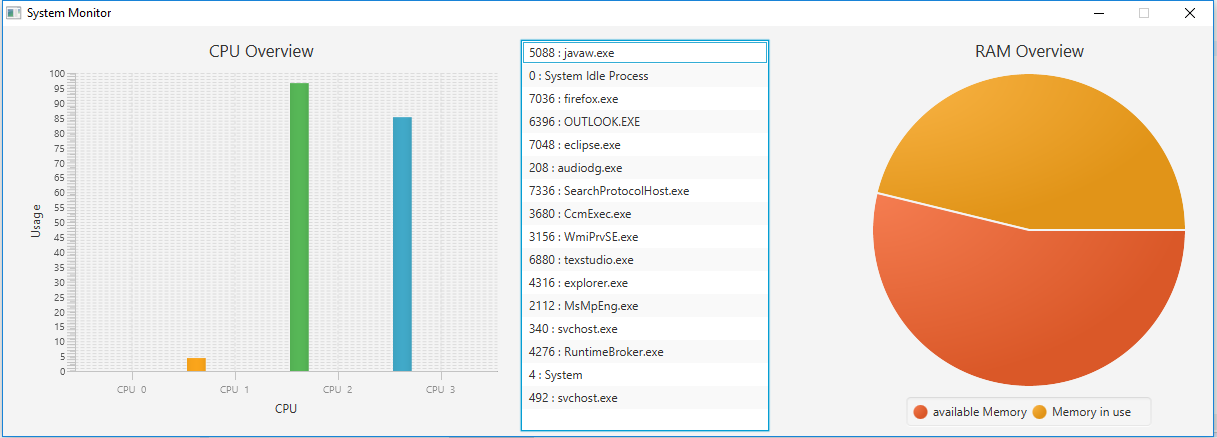
\includegraphics[width=1\textwidth]{Abb/sysmon}
	\caption{SystemMonitor Applikation}
	\label{pic:sysmon}
\end{figure}
In diesem Kapitel soll nun eine simple Anwendung beschrieben werden, die einige der zuvor geschilderten Methoden implementiert. Augenmerk liegt hier auf der Erstellung von Observables und die weitere Verwendung dieser. Als Beispiel soll ein Systemmonitor dienen. Hierfür werden die aktuelle Auslastung der Kerne, die ausgeführten Prozesse sortiert nach der CPU-Auslastung sowie der aktuell genutzte Arbeitsspeicher ausgelesen und auf einer Oberfläche dargestellt. Die Implementierung wurde mit Java 8u121 und RxJava 2.0.8 realisiert. Zusätzlich kamen noch die Bibliotheken JavaFX 8, RxJavaFX 2.0.2 sowie Oshi 3.4.0 zum Einsatz \cite{rxajavafx}, \cite{oshi}. Das Bild \ref{pic:sysmon} zeigt die fertige Applikation.
\section{Klassenbeschreibung SystemProvider}
Um sicherzustellen das die geforderten Daten des Systemmonitors verfügbar sind, wurde das ISystemProvider-Interface implementiert. 
\lstinputlisting[linerange={7-19}, float=hbt, caption={ISystemProvider-Interface}, label=lst:interface]{../SystemMonitor/src/main/java/provider/ISystemProvider.java} 
Listing \ref{lst:interface} zeigt die zu implementierenden Methoden des Interfaces. Die festen Größen, wie die Anzahl der Kerne und der verfügbare Arbeitsspeicher, werden als primitive Datentypen zur Verfügung gestellt. Die variablen Werte, also CPU-Auslastung, Prozesse und genutzter Speicher werden durch Observables repräsentiert. Die Implementierung dieser Methoden wurden in der Klasse SystemProvider vorgenommen.Verwendung findet hier das Oshi-Framework. Dieses bietet eine Schnittstelle um auf Systeminformationen außerhalb der JVM zuzugreifen. Als Einstiegspunkt dient immer ein Objekt der SystemInfo-Klasse. Dieses bietet die weiteren Informationen über das Betriebssystem oder die verwendete Hardware der Maschine. Der SystemProvider wurde als Singleton implementiert, wodurch auch nur eine Instanz der SystemInfo-Klasse verwendet wird, um die spezifischen Systeminformationen abzurufen. Interessant ist hier die Implementierung von den Methoden \textit{fetchCpuValues()}, \textit{getAvailableMemory()} und \textit{getProcesses()}. 
\subsection{List< Observable<Double> > fetchCpuValues()}
\lstinputlisting[linerange={45-56}, float=hbt, caption={SystemProvider - Implementierung der fetchCpuValues()-Methode}, label=lst:fetch]{../SystemMonitor/src/main/java/provider/SystemProvider.java} 
Die Implementierung der \textit{fetchCpuValues()}-Methode ist in Listing \ref{lst:fetch} zu sehen. Die sich ändernden Werte liegen als Double vor und repräsentieren die Stelle, welche beobachtet werden soll. Durch das Iterieren über die Anzahl der vorhandenen Kerne wird für jeden Kern ein separates Interval-Observable instanziiert. Die Taktung des Intervalls liegt bei einer Sekunde. Der vom Intervall generierte Wert wird vernachlässigt. Jedoch wird der Takt genutzt, um eine Abfrage über die aktuelle Auslastung eines Kerns durchzuführen. Bei einem 4-Kern Prozessor wird also eine Liste mit vier Observables von der Methode zurück geliefert. Da es sich um \textit{Cold Oservables} handelt, werden zu diesem Zeitpunkt noch keine Werte ausgeben. Noch zu erwähnen ist, dass ein Scheduler genutzt wird, um diesen Vorgang durchzuführen. Somit wird nicht der Thread der möglichen Subscriber verwendet, was ein Blockieren verhindern soll. 
\subsection{Observable<Long> getAvailableMemory()}
In Listing \ref{lst:memorymethod} sieht man die Implementierung der Methode um den aktuell verfügbaren Arbeitsspeicher auszulesen. Die Abfrage des Werts wird wieder mit einem Intervall durchgeführt und die Werte werden durch ein Observable repräsentiert. Auch hier wird wieder der Computation-Scheduler als Threadpool verwendet. Bis auf die Flexibilität der Kernanzahl ist das Vorgehen der Datenabfrage somit identisch zur \textit{fetchCpuValues}-Methode. Somit wird hier notwendigerweise nur ein einzelnes Observable zurück gegeben.
\lstinputlisting[linerange={64-68}, float=hbt, caption={SystemProvider - Implementierung der getAvailableMemory()-Methode}, label=lst:memorymethod]{../SystemMonitor/src/main/java/provider/SystemProvider.java} \newpage
\subsection{Observable< List<String> > getProcesses()}
\lstinputlisting[linerange={76-97}, float=hbt, caption={SystemProvider - Implementierung der getProcesses()-Methode}, label=lst:processmethod]{../SystemMonitor/src/main/java/provider/SystemProvider.java}
Die in Listing \ref{lst:processmethod} gezeigte Methode liefert ebenfalls ein Observable-Objekt zurück. Unterschied zu den beiden anderen Methoden ist hier jedoch, dass nicht nur ein Wert beobachtet wird, sondern die komplette Liste der Prozesse. Zusätzlich zum getakteten Aufruf der getProcesses()-Methode der SystemInfo-Klasse wird hier die Datenrepräsentation der Objekte geändert. Durch die Funktion \textit{func} wird aus den einzelnen Prozessen eine Liste bestehend aus der PID(ProcessID) sowie dem Prozessnamen erstellt, parametrisiert auf den Datentyp String zur einfacheren Weiterverarbeitung. Die im Observable enthaltene Liste beinhaltet 16 Prozesse sortiert nach der CPU-Auslastung. \newpage
\section{Klassenbeschreibung MainApplication}
Der bisherige Teil der Implementierung hat nur die Datenbeschaffung erledigt, es fehlt die Darstellung dieser Daten auf der Oberfläche. Hierzu dient die Klasse \textit{MainApplication}. Durch das JavaFX-Framework kann eine einfache Oberfläche implementiert werden. Durch das Erweitern der Klasse mit der abstrakten Klasse \textit{Application} des JavaFX-Frameworks, muss die \textit{start()}-Methode von der MainApplication-Klasse implementiert werden. Diese wird in der Main-Methode, welche ebenfalls in dieser Klasse untergebracht ist, aufgerufen, was zum Start der Anwendung führt. Innerhalb dieser Methode wird die Basis für die graphische Darstellung in Form der ersten \textit{Stage} gelegt. Auf dieser Stage werden alle Elemente, die dargestellt werden sollen, in einem Wurzelobjekt zusammengeführt. 
\lstinputlisting[linerange={37-51}, float=hbt, caption={MainApplication - Implementierung der start()-Methode}, label=lst:mainstart]{../SystemMonitor/src/main/java/application/MainApplication.java} 
Wie dies genau geschieht wird in Listing \ref{lst:mainstart} beschrieben. Mit der BorderPane als Basislayout wird ein Wurzelelement der Oberfläche geschaffen. Darauf werden horizontal angeordnet die eigentlichen Knoten(Nodes) festgelegt. Die Anordnung wird durch die verwendete \textit{HBox} übernommen. Die statischen Methoden \textit{createBarChart()}, \textit{createProcessList()} und \textit{createPieChart()} sind die Methoden, auf welche das eigentliche Augenmerk gerichtet wird, denn in diesen Methoden werden die Observables der vorangegangenen SystemProvider-Klasse verwendet. 
\subsection{Node createBarChart()}
\lstinputlisting[linerange={53-55, 68-79}, float=hbt, caption={MainApplication - Auszug aus der Implementierung der createBarChart()-Methode}, label=lst:barchartmethod]{../SystemMonitor/src/main/java/application/MainApplication.java} 
Diese Methode liefert einen Knoten von Typ BarChart(Balkendiagramm) zurück. Die BarChart arbeitet mit Serien von Daten die innerhalb des Diagramms dargestellt werden. Jede Serie besteht wiederum aus eine Menge von Daten mit jeweils einem \textit{x} und einem \textit{y} Wert. Die Serien werden von dem BarChart-Objekt in einer \textit{ObservableList} verwaltet. Dieser Datentyp stammt aus der JavaFX-Bibliothek und bietet die Möglichkeit die Liste von Daten zu beobachten und bei Änderung zu reagieren. Die Reihenfolge der Beobachtung der Datenänderungen ist gestaffelt. Für jedes Observable welches einen Kern und somit dessen aktuelle Auslastung repräsentiert, wird in einer separaten Serie gespeichert. Jede dieser Serien enthält einen Datensatz. In der Hilfsmethode \textit{setObservableChartData()} wird dieser Schritt durchgeführt wie es auch in Listing \ref{lst:helpermethod} dargestellt ist. 
\lstinputlisting[linerange={ 81-90}, float=hbt, caption={MainApplication - zusätzliche Hilfmethode setObservableChartData()}, label=lst:helpermethod]{../SystemMonitor/src/main/java/application/MainApplication.java} 
Der verantwortliche Datensatz der Serie subscribed dem Observable welches den aktuellen CPU-Wert propagiert. Somit enthält die Serie eine Datensatz mit sich ständig ändernden Daten. Diese Serie wird nun in der ObservableList abgelegt. Sind Serien für jeden der Kerne erstellt, wird die Liste als Datensatz dem Balkendiagramm übergeben. Findet nun eine Wertänderung statt, wird diese auf dem \textit{JavaFxScheduler.platform()}-Thread ausgeführt. Dieser Thread repräsentiert die Änderungen auf der Oberfläche. Somit wird bei jeder Wertänderung die Serie des Balkendiagramms aktualisiert. Die Implementierung der \textit{createBarChart()}-Methode und die Verwendung der Hilfsmethode zeigt Listing \ref{lst:barchartmethod}. In der \textit{for()}-Schleife wird für jeden Kern die Hilfsmethode ausgeführt und eine Serie mit Daten zurück geliefert. Diese wird der ObservableList hinzugefügt, welche wiederum als Datensatz des BarCharts verwendet wird.
\subsection{Node createPieChart()}
\lstinputlisting[linerange={92-94,101-105, 107-111, 114-115}, float=hbt, caption={MainApplication - Auszug aus der Implementierung der createPieChart()-Methode}, label=lst:piechartmethod]{../SystemMonitor/src/main/java/application/MainApplication.java} 
Die Auslastung des RAM wird als PieChart(Kreisdiagramm) dargestellt. Auch hier werden die Daten wieder in einer ObservableList parametrisiert auf den Datentyp Data abgelegt, welcher von der PieChart-Bibliothek zur Verfügung gestellt wird. In diesem Beispiel besteht der Kreis nur aus zwei Werten, dem genutzten und dem noch verfügbaren RAM. Das Observable erhält die Methode des SystemProviders über die Verwendung der SystemProvider-Instanz. Da die beiden Werte immer zusammen den Kreis komplett ausfüllen, also 100\% des RAM repräsentieren, werden die beiden Werte in einer Subscription aktualisiert. Auch hier erhält das PieChart die ObservableList mit den beiden Werten. Die Wertänderung wird wieder auf dem JavaFxScheduler-Threadpool ausgeführt, um die Wertänderungen an die GUI zu publizieren. Listing \ref{lst:piechartmethod} zeigt diese Implementierung. Als Node für die GUI wird die PieChart von der Methode zurückgegeben.
\subsection{Node createProcessList()}
\lstinputlisting[linerange={117-125}, float=hbt, caption={MainApplication - Implementierung der createProcesses()-Methode}, label=lst:getprocessesmethod]{../SystemMonitor/src/main/java/application/MainApplication.java}
Die Prozessliste wird von einem Node des Types ListView(Listenansicht) auf der Benutzeroberfläche repräsentiert. Die \textit{getProcesses()}-Methode des Systemproviders liefert wieder das Observable, was jede Sekunde die Liste der Prozesse über das Oshi-Framework abfragt. Die Beobachtung findet über die vollständige Liste statt, somit findet auch die Subscription an diesem Observable-Objekt statt. Die Daten der ListView werden ebenfalls in einer ObservableList verwaltet. Innerhalb der Subscription wird somit die Liste des Providers in eine ObservableList transformiert und als Einträge in die ListView hinzugefügt. 
Die konkrete Implementierung findet sich in Listing \ref{lst:getprocessesmethod}.
\section{Beschreibung des Beispiels}
Das Beispiel implementiert mehrere Methoden nach den Prinzipien des Reactive Programming. Die Systeminformationen werden über die vom Oshi-Framework zu Verfügung stehenden Methoden bezogen. Dies geschieht nach dem Pull-Verfahren, also für jede Abfrage der Daten muss ein separater Aufruf der Methode stattfinden. Hierfür dient die Instanziierung der Observables als Intervall. Diese Observables werden alle in einem Thread des RxJava eigenen \textit{Schedulers.computation()} Threadpool gestartet, sobald eine Subscription registriert wird. Somit handelt es sich hier um Cold Observables. Betrachtet man die Methode für das Erstellen der Observables für die Auslastung der einzelnen Kerne stellt man fest, dass die Intervalle unabhängig voneinander starten. Somit findet die Aktualisierung der Werte der unterschiedlichen Kerne asynchron und nebenläufig statt. Die Datenaktualisierung der GUI muss auf dem MainThread der JavaFX-Application ausgeführt werden. Um diesen Thread nur für die vorgesehenen Aktualisierungen zu verwenden, wird bei jeder der Methoden zum Erstellen der unterschiedlichen Nodes der \textit{JavaFxScheduler.platform()} Threadpool verwendet und zwar nur für die relevanten Datenänderungen und nicht für zusätzliche, von der GUI unabhängige, Aufgaben. Somit muss die Funktionalität der \textit{observOn()}-Methode für die jeweilige Subscription genutzt werden, sodass die Berechnung und Datenbeschaffung außerhalb und die Änderung der beobachteten Daten der Oberflächenelemente innerhalb des MainThreads der Application ausgeführt werden. Durch die Vielfalt der RxJava-Bibliothek kann dieses Beispiel nur einige Aspekte dieser Bibliothek abdecken, veranschaulicht aber zumindest den grundsätzlichen Umgang mit Observables innerhalb einer Applikation.
	

\bibliographystyle{alphadin}
\bibliography{literatur}
\pagenumbering{Roman}	
	
% ----- Abbildungen ----- %
%\addcontentsline{toc}{section}{Abbildungsverzeichnis} % falls in Inhalsverzeichnis
\listoffigures

% ----- Tabellen----- %
% \addcontentsline{toc}{section}{Tabellenverzeichnis}  % falls in Inhalsverzeichnis
% \fancyhead[L]{Abbildungsverzeichnis / Abkürzungsverzeichnis} %Kopfzeile links
\listoftables

% ----- Listings ----- %
% Listingverzeichnis soll im Inhaltsverzeichnis auftauchen
% \addcontentsline{toc}{section}{Listingverzeichnis}
% \fancyhead[L]{Abbildungs- / Tabellen- / Listingverzeichnis} %Kopfzeile links
\renewcommand{\lstlistlistingname}{Listingverzeichnis}
\lstlistoflistings
	
\end{document}